\section{ASP.NET Core}
ASP.NET Core is a web framework developed by Microsoft, for developing web applications in the .NET Core framework.
The framework is quite widely used, which means that there are plenty of modules available for doing many jobs. Besides that, the framework has built-in support for many common features, such as database integration, identity and authorization with multi-factor and external auth, CSS frameworks, and much more.
It uses the quite popular Model-View-Controller design pattern as a basis for the architecture of the applications developed in it.
\subsection{Model-View-Controller design pattern}
The Model-View-Controller pattern is an architectural pattern that splits the application into three basic components, the model, the view, and the controller. Originally meant for GUI development, the pattern has been adapted into web development, and is used by many of the frameworks in the space.\cite{gangoffour}

\begin{figure}[H]
\centering
	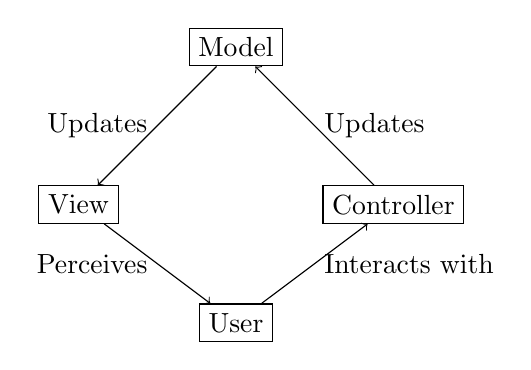
\begin{tikzpicture}[node distance=2cm]
	\node[draw] (model) {Model};
	\node[draw] (view) [below of=model, left of=model] {View};
	\node[draw] (controller) [below of=model, right of=model] {Controller};
	\draw[->] (model) -- node[left] {Updates} (view);
	\draw[->] (controller) -- node[right] {Updates} (model);
	\node[draw] (user) [below of=model, node distance=3.5cm] {User};
	\draw[->] (view) -- node[left] {Perceives} (user);
	\draw[->] (user) -- node[right] {Interacts with} (controller);
	\end{tikzpicture}
	\caption{The Model-View-Controller design pattern.}
\end{figure}

The basic idea of the pattern is that all of the data managed by the application is encapsulated into the model classes.
These can then be accessed or subscribed to by the views, which the user sees.
The user then subsequently interacts with the controller, which in turn updates the model.
The seperation of concerns allows for a quite flexible architecture, where you can change the view without touching the model or controller, or the controller without changing the view and model.\cite{gangoffour}
\subsection{Entity Framework}
\todo[inline]{We need to discuss the placement of this section, in regards to the placement of the database chapter.}
Entity Framework is a framework for mapping object-oriented data structures into a relational database, also referred to an object-relational mapping framework, for .NET.\cite{efcore}
The job of the Entity Framework is translating the objects in memory into SQL statements so that these objects can be stored in a database.
\begin{figure}[H]
	\centering
	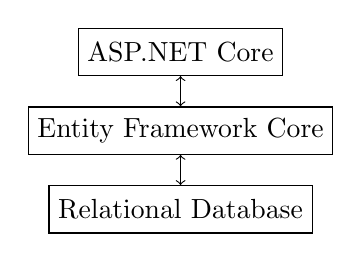
\begin{tikzpicture}[node distance=1cm, minimum height=0.6cm]
		\node[draw] (net) {ASP.NET Core};
		\node[draw] (efcore) [below of=net] {Entity Framework Core};
		\node[draw] (sql) [below of=efcore] {Relational Database};
		\draw[->] (net) -- (efcore);
		\draw[->] (efcore) -- (net);
		\draw[->] (sql) -- (efcore);
		\draw[->] (efcore) -- (sql);
	\end{tikzpicture}
	\caption{The relationship between ASP.NET Core and the Relational Database, with the Entity Framework acting as a glue between the two layers}
\end{figure}
To use the Entity Framework, all you need to do in the code is to provide a context object, which mediates this connection, giving the configuration arguments a connection to a database requires.
This context defines the sets of objects to be stored in the database, and also the database to be used.
The Entity Framework supports multiple kinds of relational databases, from MariaDB to PostgreSQL.
The support for multiple database systems are provided by the respective database providers.
